\documentclass[12pt]{article}
\usepackage[
  top=2.50cm,
  bottom=1.50cm,
  left=1.50cm,
  right=1.50cm
]{geometry} 
\usepackage{amsmath,amsthm,amssymb}
\usepackage{algorithm,algorithmic}
\usepackage{graphicx}

\newenvironment{theorem}[2][Theorem]{\begin{trivlist}
\item[\hskip \labelsep {\bfseries #1}\hskip \labelsep {\bfseries #2.}]}{\end{trivlist}}
\newenvironment{lemma}[2][Lemma]{\begin{trivlist}
\item[\hskip \labelsep {\bfseries #1}\hskip \labelsep {\bfseries #2.}]}{\end{trivlist}}
\newenvironment{exercise}[2][Exercise]{\begin{trivlist}
\item[\hskip \labelsep {\bfseries #1}\hskip \labelsep {\bfseries #2.}]}{\end{trivlist}}
\newenvironment{problem}[2][Problem]{\begin{trivlist}
\item[\hskip \labelsep {\bfseries #1}\hskip \labelsep {\bfseries #2.}]}{\end{trivlist}}
\newenvironment{question}[2][Question]{\begin{trivlist}
\item[\hskip \labelsep {\bfseries #1}\hskip \labelsep {\bfseries #2.}]}{\end{trivlist}}
\newenvironment{corollary}[2][Corollary]{\begin{trivlist}
\item[\hskip \labelsep {\bfseries #1}\hskip \labelsep {\bfseries #2.}]}{\end{trivlist}}

\begin{document}

\title{Homework 1}
\author{Thomas Kim~tsk389\\David Munoz~dam2989\\
CS331 Algorithms and Complexity}

\renewcommand{\arraystretch}{2.0}

\date{} % Suppress the datn{minipage}{0.5\textwidth}

% ------------------
% Begin Cover Page
% ------------------

\maketitle
% ------------------
% Begin Homework
% ------------------

\onecolumn

\begin{problem}
  {Q1(a)}
    Sort the following list of functions in ascending order of growth rates.\\
    % TODO: order these
      \begin{enumerate}
        \item $f_7(n) = \sqrt{n}$
        \item $f_4(n) = n(logn)^3$
        \item $f_5(n) = n^4$
        \item $f_6(n) = 2^{2^{log(logn)}}$
        \item $f_3(n) = n^{logn}$
        \item $f_2(n) = 2^{n^3}$
        \item $f_1(n) = 2^{2^n}$
      \end{enumerate}
\end{problem}

\begin{problem}
  {Q1(b)}
  Consider a network $G = (V,E)$ with a source $s$, a sink $t$, and a capacity $c_e$ on every edge $e \in E$. \\
  Claim: if $f$ is a maximum $s-t$ flow in $G$, then $f$ either saturates every edge out of $s$ or saturates every edge into $t$. \\
  \textbf{False} \\
  \begin{proof}
  \begin{center}
  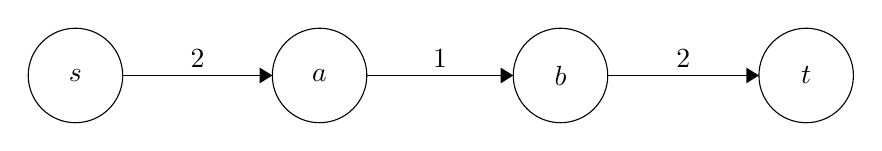
\begin{tikzpicture}[scale=0.2]
  \tikzstyle{every node}+=[inner sep=0pt]
  \draw [black] (8.5,-30.9) circle (3);
  \draw (8.5,-30.9) node {$s$};
  \draw [black] (24,-30.9) circle (3);
  \draw (24,-30.9) node {$a$};
  \draw [black] (39.3,-30.9) circle (3);
  \draw (39.3,-30.9) node {$b$};
  \draw [black] (54.9,-30.9) circle (3);
  \draw (54.9,-30.9) node {$t$};
  \draw [black] (11.5,-30.9) -- (21,-30.9);
  \fill [black] (21,-30.9) -- (20.2,-30.4) -- (20.2,-31.4);
  \draw (16.25,-30.4) node [above] {$2$};
  \draw [black] (27,-30.9) -- (36.3,-30.9);
  \fill [black] (36.3,-30.9) -- (35.5,-30.4) -- (35.5,-31.4);
  \draw (31.65,-30.4) node [above] {$1$};
  \draw [black] (42.3,-30.9) -- (51.9,-30.9);
  \fill [black] (51.9,-30.9) -- (51.1,-30.4) -- (51.1,-31.4);
  \draw (47.1,-30.4) node [above] {$2$};
  \end{tikzpicture}
  \end{center}
  The min cut is $A = \{s,a\}, B = \{b,t\}$. The value of this cut is $1$, which implies the max flow $f = 1$. This does not saturate the edge leaving $s$ or the edge entering $t$. \\
  \end{proof}
\end{problem}

\begin{problem}
  {Q1(c)}
  Prove the following using induction for every $a \ne 1$ \\
  \begin{align*}
    \sum_{i=0}^{n-1}a^i = \frac{1 - a^n}{1-a}
  \end{align*}
  \begin{proof}
    \textbf{Base case:} \\
    \begin{align*}
    \sum_{i=0}^{n-1}2^i \\
    \sum_{i=0}^{n-x}2^i = (2\sum_{i = 0}^{n-x}2^i) + 1\\
    \sum_{i=0}^{n-1}2^i = 2^{n-1} + 2^{n-1} - 1 \\
    =2(2^{n-1}) - 1 = 2^{n} - 1 \\
    =-(2^{n} - 1) / (-1) = \frac{1 - 2^n}{(1 - 2)} \\
    \end{align*}
    \textbf{Induction Hypothesis:} \\
  \end{proof}
\end{problem}

\begin{problem}
  {Q2(a)}
  Briefly explain which steps of Dijkstra's algorithm fail when a graph can have negative weight edges. \\\\
  \textbf{Actual answer}: \\
  Dijkstra's algorithm relies on a breadth-first search using a priority queue and stops execution when the goal is reached. \\
  The stopping of execution when the goal has been reached relies on the invariant that the current path is the shortest path found
  so far, and that any other paths will either increase or stay the same in cost if explored. \\
  However, negative-weight edges can result in the cost of a path being explored to decrease, violating this invariant. \\
  This problem can be trivially solved by simply running BFS until all vertices are explored. \\
\end{problem}

\begin{problem}
    {Q2(b)}
    Assumptions: No driver has an empty list. \\\\
    Basic premise: \\
    1. Group together drivers who (transitively) share a bus with another driver in the group. \\
    2. Connect that group with the set of buses that are collectively shared (set union of all their lists). \\
    3. If the group size is larger than the number of buses it maps to, give the drivers GPSes
    4. Otherwise put them on the buses which correspond to the group. \\\\
    To solve (1), simply connect drivers who share a bus with an edge, then take each connected component as a group. \\
    \noindent
    \textbf{Runtime}
    \begin{proof}
        Constructing the graph for step (1) takes $O(n^2)$ time, as there are $n+1$ lists each with up to $n+1$ buses on them \\
        Finding connected components can be done in polynomial time using BFS or DFS. \\
        The final assignment of GPSes can be done in $O(n)$ time, as each driver and bus is considered exactly once. \\
        The runtime is therefore polynomial in $n$. \\
    \end{proof}
    \noindent
    \textbf{Correctness}
    \noindent
    \textbf{Pf. of Validity}
    \begin{proof}
        The set union of all groups is equal to the set of all drivers. \\
        Since each group maps to some set of buses, and either the entire group or entire mapped buses get GPS, the matching is valid. \\
    \end{proof}
    \noindent
    \textbf{Pf. of Optimality}
    \begin{proof}
        Suppose some group is given GPSes but it would be more ideal to give GPSes to their mapped buses. \\
        Note that no other group can be mapped to any of these buses by construction, otherwise this group would be part of another group. \\
        This implies there are fewer buses than people. \\
        This is a contradiction, as step 3 of the algorithm implies there are fewer drivers in the group than mapped buses. \\
        Suppose some mapped buses are given GPSes but it would be more ideal to give GPSes to the group mapped to them. \\
        Note that by the pigeonhole principle, at least one driver will be idle at any given time. \\
        This means giving a GPS to that driver will cause one idle GPS at any time. \\
        However, if all those GPSes were given to the buses, then there would be 0 idle GPSes, as there are more drivers than buses by line 4. \\
    \end{proof}
\end{problem}

\begin{problem}
    {Q3}
    Show that the following problem is undecidable. \\
    \begin{align*}
        \textbf{A} = \{<M> | \forall w \in \textbf{S}~M \text{accepts} w\} \text{ where \textbf{S} is the set of all strings}
    \end{align*}
    \begin{proof}
        Define a mapping reduction $R(<M>)$ as follows: \\\\
        1. Erase the tape \\
        2. Write $\epsilon$ to the tape \\
        3. Run $M$ on $\epsilon$ \\
        4. Accept \\
        Return $<M\#>$ \\\\
        %% TODO: Not sure what we're allowed to reduce to
        If $<M> \in H_\epsilon: M$ halts on $\epsilon$, so $M\#$ accepts everything. Oracle $<M\#>$ accepts. \\
        If $<M> \not\in H_\epsilon: M$ does not halt on $\epsilon$, so $M\#$ accepts nothing and doesn't halt. Oracle $<M\#>$ rejects. \\
        However, no machine to decide $H$ can exist, so Oracle doesn't exist. \\
    \end{proof}
\end{problem}


% -----------------
% End Homework
% -----------------

\end{document}
